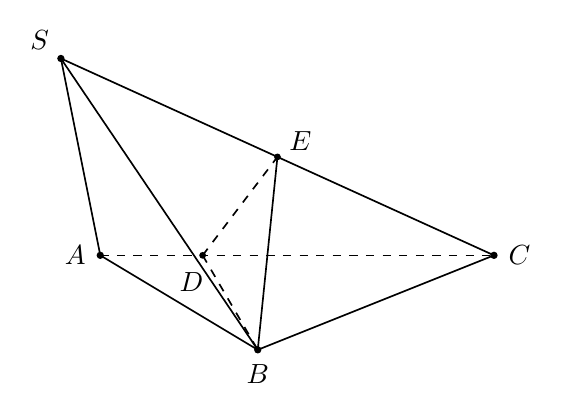
\begin{tikzpicture}[x=1cm,y=1cm,line width=0.6pt]
\tikzset{ptlabel/.style={font=\normalsize,fill=white,inner sep=1pt}}
\coordinate (S) at (-2.5,2.5);
\coordinate (A) at (-2,0);
\coordinate (C) at (3,0);
\coordinate (B) at (0,-1.2);
\coordinate (E) at (0.25,1.25);
\coordinate (D) at (-0.7,0);
% base AC dashed
\draw[draw=black,dashed] (A) -- (C);
% solid skeleton
\draw[draw=black] (S) -- (A);
\draw[draw=black] (S) -- (C);
\draw[draw=black] (S) -- (B);
\draw[draw=black] (A) -- (B);
\draw[draw=black] (B) -- (C);
\draw[draw=black] (B) -- (E);
% dashed interior
\draw[draw=black,dashed] (D) -- (E);
\draw[draw=black,dashed] (D) -- (B);
% markers
\filldraw[draw=black,fill=black] (S) circle (1pt);
\filldraw[draw=black,fill=black] (A) circle (1pt);
\filldraw[draw=black,fill=black] (B) circle (1pt);
\filldraw[draw=black,fill=black] (C) circle (1pt);
\filldraw[draw=black,fill=black] (D) circle (0.9pt);
\filldraw[draw=black,fill=black] (E) circle (0.9pt);
% labels with clearance
\node[ptlabel,anchor=south east,xshift=-3pt,yshift=2pt] at (S) {$S$};
\node[ptlabel,anchor=east,xshift=-4pt] at (A) {$A$};
\node[ptlabel,anchor=west,xshift=4pt] at (C) {$C$};
\node[ptlabel,anchor=north,yshift=-4pt] at (B) {$B$};
\node[ptlabel,anchor=south west,xshift=3pt,yshift=1pt] at (E) {$E$};
\node[ptlabel,anchor=north,yshift=-5pt,fill=none,xshift=-4.00bp,yshift=0.00bp] at (D) {$D$};
\end{tikzpicture}
